
%%%%%%%%%%%%%%%%%%%%%%%%%%%%%%%%%%%%%%%%%%%%%%%%%%%%%%%%%%%%%%%%%%%%%%%%%%%%%%
% Copyright (c) 2003-2015 by University of Queensland
% http://www.uq.edu.au
%
% Primary Business: Queensland, Australia
% Licensed under the Open Software License version 3.0
% http://www.opensource.org/licenses/osl-3.0.php
%
% Development until 2012 by Earth Systems Science Computational Center (ESSCC)
% Development 2012-2013 by School of Earth Sciences
% Development from 2014 by Centre for Geoscience Computing (GeoComp)
%
%%%%%%%%%%%%%%%%%%%%%%%%%%%%%%%%%%%%%%%%%%%%%%%%%%%%%%%%%%%%%%%%%%%%%%%%%%%%%%

\section{Newtonian Potential}

In this chapter the gravitational potential field is developed for \esc.
Gravitational fields are present in many modelling scenarios, including
geophysical investigations, planetary motion and attraction and micro-particle
interactions. Gravitational fields also present an opportunity to demonstrate
the saving and visualisation of vector data for Mayavi, and the construction of
variable sized meshes.

The gravitational potential $U$ at a point $P$ due to a region with a mass
distribution of density $\rho(P)$, is given by Poisson's equation
\citep{Blakely1995}
\begin{equation} \label{eqn:poisson}
\nabla^2 U(P) = -4\pi\gamma\rho(P)
\end{equation}
where $\gamma$ is the gravitational constant.
Consider now the \esc general form, 
\autoref{eqn:poisson} requires only two coefficients,
$A$ and $Y$, thus the relevant terms of the general form are reduced to;
\begin{equation}
-\left(A_{jl} u_{,l} \right)_{,j} = Y
\end{equation}
One recognises that the LHS side is equivalent to 
\begin{equation} \label{eqn:ex10a}
-\nabla A \nabla u
\end{equation}
and when $A=\delta_{jl}$, \autoref{eqn:ex10a} is equivalent to
\begin{equation*}
-\nabla^2 u
\end{equation*}
Thus Poisson's \autoref{eqn:poisson} satisfies the general form when
\begin{equation}
A=\delta_{jl} \text{ and } Y= 4\pi\gamma\rho
\end{equation}
The boundary condition is the last parameter that requires consideration. The
potential $U$ is related to the mass of a sphere by
\begin{equation}
U(P)=-\gamma \frac{m}{r^2}
\end{equation} where $m$ is the mass of the sphere and $r$ is the distance from
the center of the mass to the observation point $P$. Plainly, the magnitude
of the potential is governed by an inverse-square distance law. Thus, in the
limit as $r$ increases;
\begin{equation}
\lim_{r\to\infty} U(P) = 0
\end{equation}
Provided that the domain being solved is large enough, and the source mass is
contained within a central region of the domain, the potential will decay to
zero. This is a dirichlet boundary condition where $U=0$.

This boundary condition can be satisfied when there is some mass suspended in a
free-space. For geophysical models where the mass of interest may be an anomaly
inside a host rock, the anomaly can be isolated by subtracting the density of the
host rock from the model. This creates a fictitious free space model that will
satisfy the analytic boundary conditions. The result is that
$Y=4\pi\gamma\Delta\rho$, where $\Delta\rho=\rho-\rho_0$ and $\rho_0$ is the
baseline or host density. This of course means that the true gravity response is
not being modelled, but the response due to an anomalous mass with a
density contrast $\Delta\rho$.

For this example we have set all of the boundaries to zero but only one boundary
point needs to be set for the problem to be solvable. The normal flux condition
is also zero by default. Note, that for a more realistic and complicated models
it may be necessary to give careful consideration to the boundary conditions of the model,
which can have an influence upon the solution.

Setting the boundary condition is relatively simple using the \verb!q! and
\verb!r! variables of the general form. First \verb!q! is defined as a masking
function on the boundary using
\begin{python}
q=whereZero(x[1]-my)+whereZero(x[1])+whereZero(x[0])+whereZero(x[0]-mx)
mypde.setValue(q=q,r=0)
\end{python}
This identifies the points on the boundary and \verb!r! is simply
ser to \verb!r=0.0!. This is a Dirichlet boundary condition.

\clearpage
\section{Gravity Pole}
\sslist{example10a.py}
A gravity pole is used in this example to demonstrate the vector characteristics
of gravity, and also to demonstrate how this information can be exported for
visualisation to Mayavi or an equivalent using the VTK data format.

The solution script for this section is very simple. First the domain is
constructed, then the parameters of the model are set, and finally the steady
state solution is found. There are quite a few values that can now be derived
from the solution and saved to file for visualisation.

The potential $U$ is related to the gravitational response $\vec{g}$ via
\begin{equation}
\vec{g} = \nabla U
\end{equation}
$\vec{g}$ is a vector and thus, has a a vertical component $g_{z}$ where
\begin{equation}
g_{z}=\vec{g}\cdot\hat{z}
\end{equation}
Finally, there is the magnitude of the vertical component $g$ of
$g_{z}$
\begin{equation}
g=|g_{z}|
\end{equation}
These values are derived from the \esc solution \verb!sol! to the potential $U$
using the following commands
\begin{python}
g_field=grad(sol) #The gravitational acceleration g.
g_fieldz=g_field*[0,1] #The vertical component of the g field.
gz=length(g_fieldz) #The magnitude of the vertical component.
\end{python}
This data can now be simply exported to a VTK file via
\begin{python}
# Save the output to file.
saveVTK(os.path.join(save_path,"ex10a.vtu"),\
        grav_pot=sol,g_field=g_field,g_fieldz=g_fieldz,gz=gz)
\end{python}

It is quite simple to visualise the data from the gravity solution in Mayavi2.
With Mayavi2 open go to File, Load data, Open file \ldots as in
\autoref{fig:mayavi2openfile} and select the saved data file. The data will
have then been loaded and is ready for visualisation. Notice that under the data
object in the Mayavi2 navigation tree the 4 values saved to the VTK file are
available (\autoref{fig:mayavi2data}). There are two vector values,
\verb|gfield| and \verb|gfieldz|. Note that to plot both of these on the same
chart requires that the data object be imported twice.

The point scalar data \verb|grav_pot| is the gravitational potential and it is
easily plotted using a surface module. To visualise the cell data a filter is
required that converts to point data. This is done by right clicking on the data
object in the explorer tree and selecting the cell to point filter as in
\autoref{fig:mayavi2cell2point}.

The settings can then be modified to suit personal taste. An example of the
potential and gravitational field vectors is illustrated in
\autoref{fig:ex10pot}.

\begin{figure}[ht]
\centering
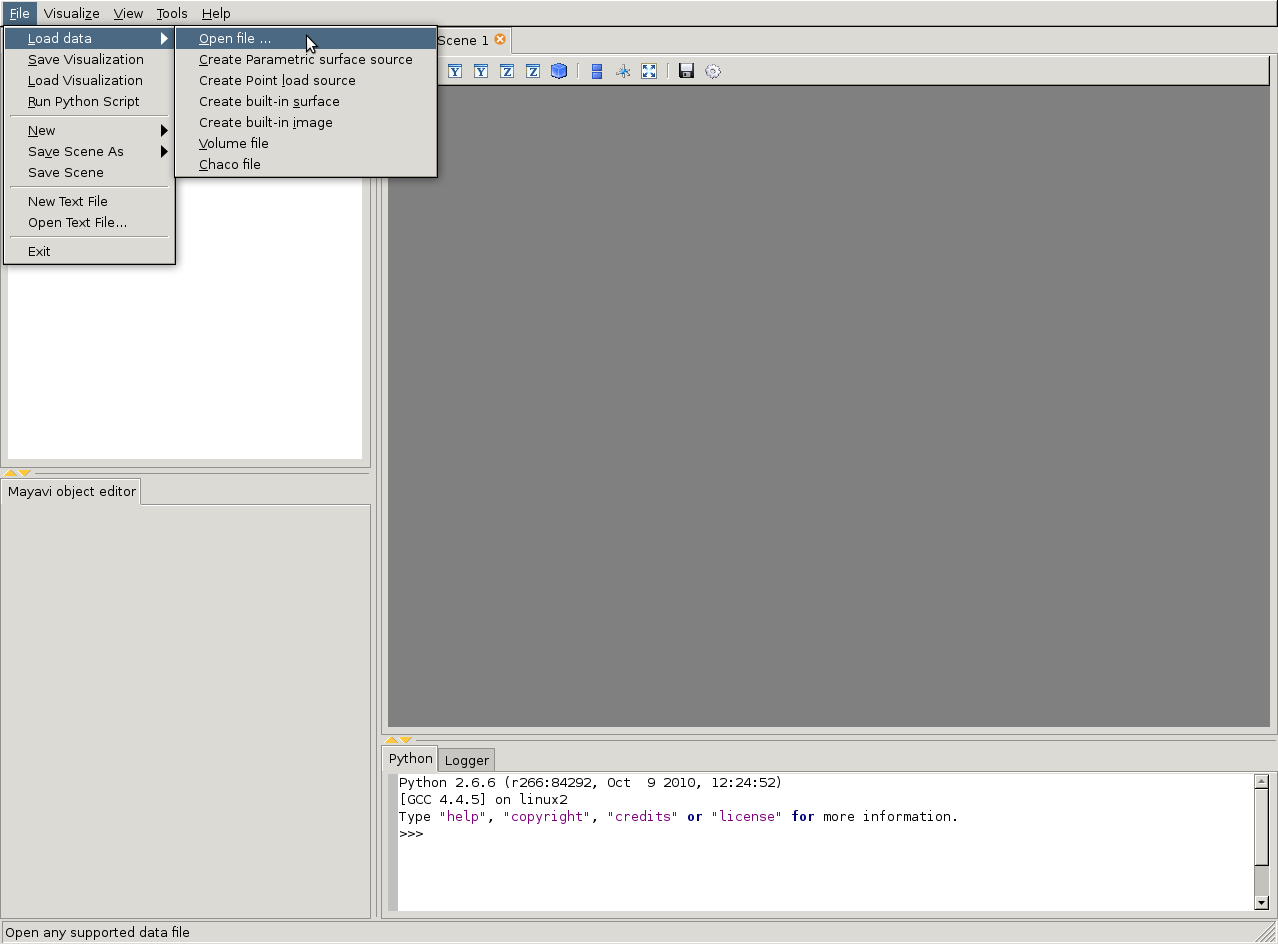
\includegraphics[width=0.75\textwidth]{figures/mayavi2_openfile.png}
\caption{Open a file in Mayavi2}
\label{fig:mayavi2openfile}
\end{figure}

\begin{figure}[ht]
\centering
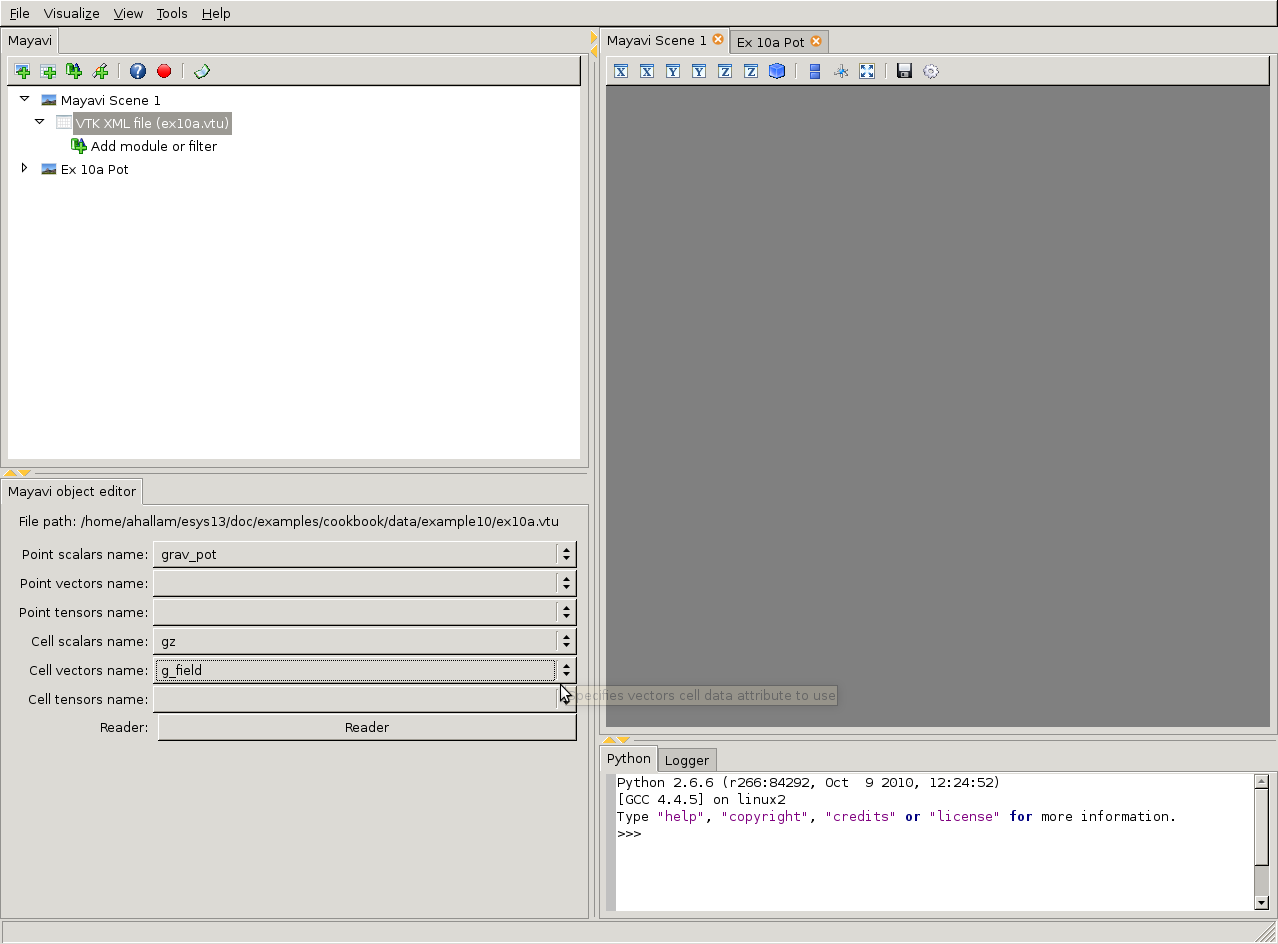
\includegraphics[width=0.75\textwidth]{figures/mayavi2_data.png}
\caption{The 4 types of data in the imported VTK file.}
\label{fig:mayavi2data}
\end{figure}

\begin{figure}[ht]
\centering
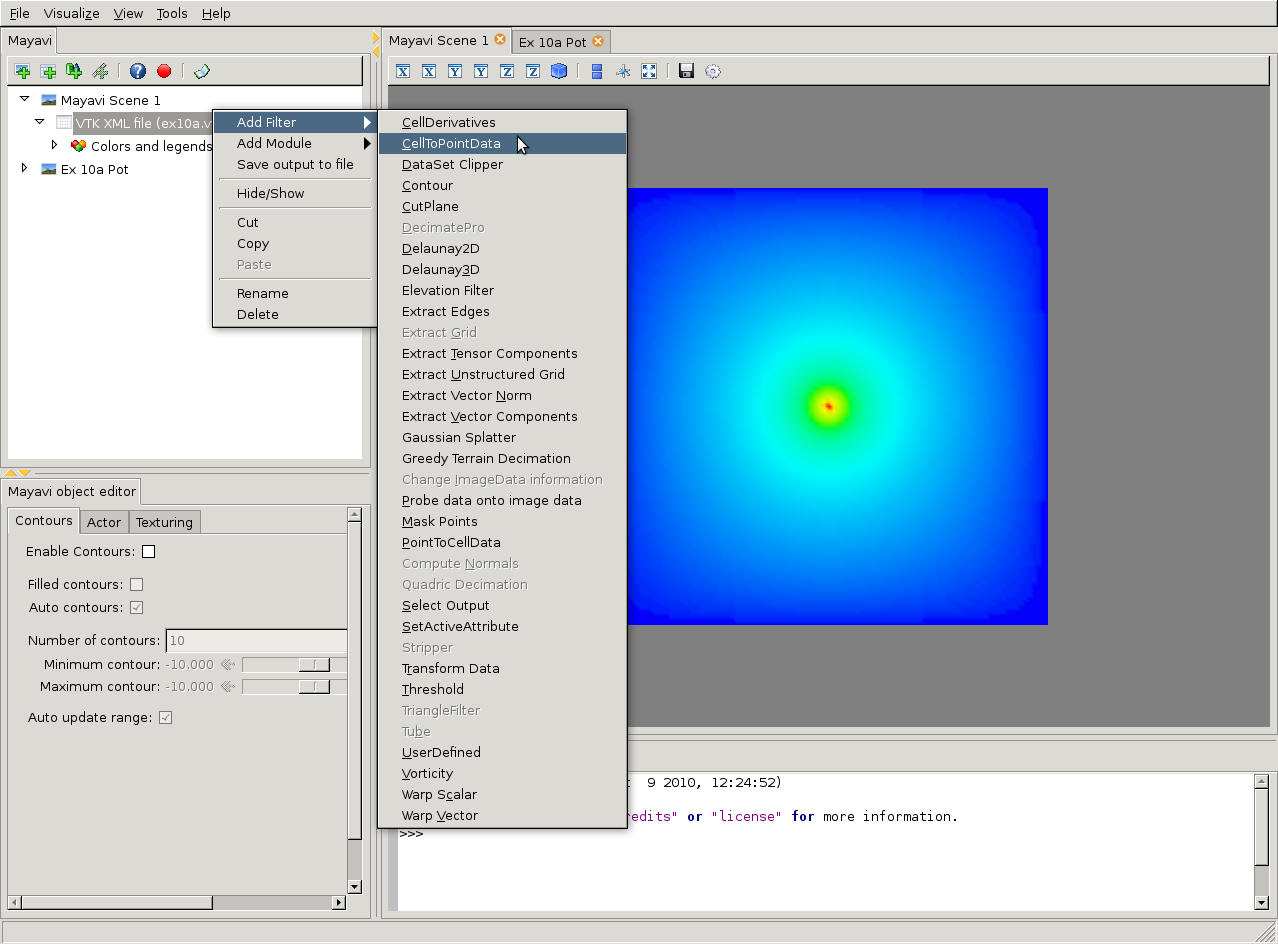
\includegraphics[width=0.75\textwidth]{figures/mayavi2_cell2point.png}
\caption{Converting cell data to point data.}
\label{fig:mayavi2cell2point}
\end{figure}

\begin{figure}[ht]
\centering
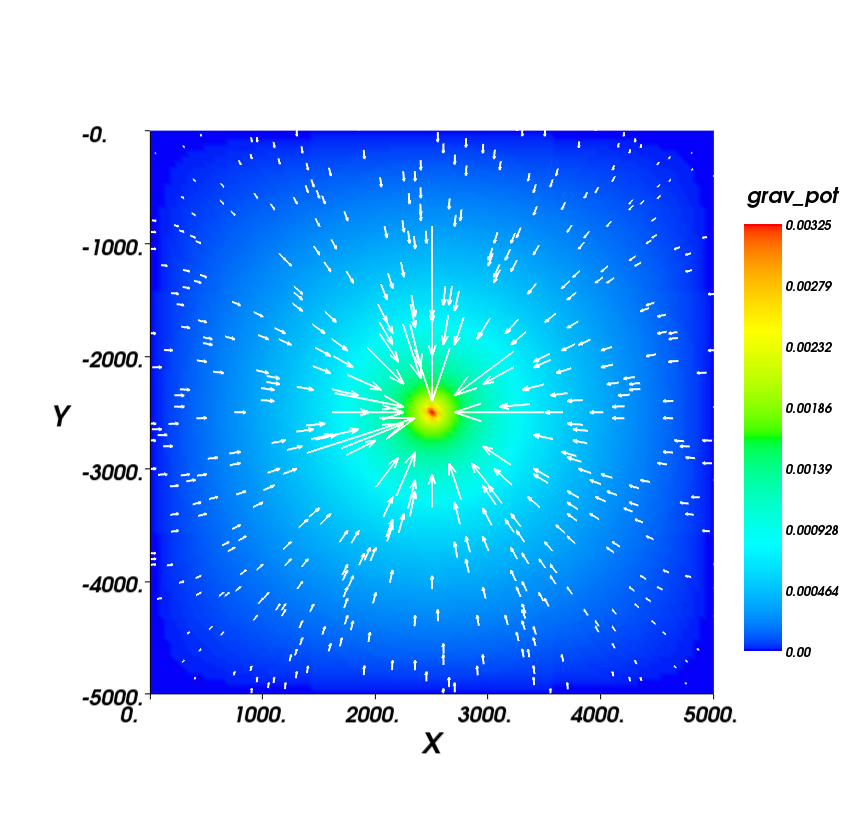
\includegraphics[width=0.75\textwidth]{figures/ex10apot.png}
\caption{Newtonian potential with $\vec{g}$ field directionality. The magnitude
of the field is reflected in the size of the vector arrows.}
\label{fig:ex10pot}
\end{figure}
\clearpage

\section{Gravity Well}
\sslist{example10b.py}
Let us now investigate the effect of gravity in three dimensions. Consider a
volume which contains a spherical mass anomaly and a gravitational potential
which decays to zero at the base of the model.

The script used to solve this model is very similar to that used for the gravity
pole in the previous section, but with an extra spatial dimension. As for all
the 3D problems examined in this cookbook, the extra dimension is easily
integrated into the \esc solution script.

The domain is redefined from a rectangle to a Brick;
\begin{python}
domain = Brick(l0=mx,l1=my,n0=ndx, n1=ndy,l2=mz,n2=ndz)
\end{python}
the source is relocated along $z$;
\begin{python}
x=x-[mx/2,my/2,mz/2]
\end{python}
and, the boundary conditions are updated.
\begin{python}
q=whereZero(x[2]-inf(x[2]))
\end{python}
No modifications to the PDE solution section are required. Thus the migration
from a 2D to a 3D problem is almost trivial.

\autoref{fig:ex10bpot} illustrates the strength of a PDE solution. Three
different visualisation types help define and illuminate properties of the data.
The cut surfaces of the potential are similar to a 2D section for a given x or y
and z. The iso-surfaces illuminate the 3D shape of the gravity field, as well as
its strength which is illustrated by the colour. Finally, the streamlines
highlight the directional flow of the gravity field in this example.

The boundary conditions were discussed previously, but not thoroughly
investigated. It was stated, that in the limit as the boundary becomes more
remote from the source, the potential will reduce to zero.
\autoref{fig:ex10bpot2} is the solution to the same gravity problem
but with a slightly larger domain. It is obvious in this case that
the previous domain size was too small to accurately represent the
solution. The profiles in \autoref{fig:ex10p} further demonstrates the affect
the domain size has upon the solution. As the domain size increases, the
profiles begin to converge. This convergence is a good indicator of an
appropriately dimensioned model for the problem, and and sampling location. 

\begin{figure}[htp]
\centering
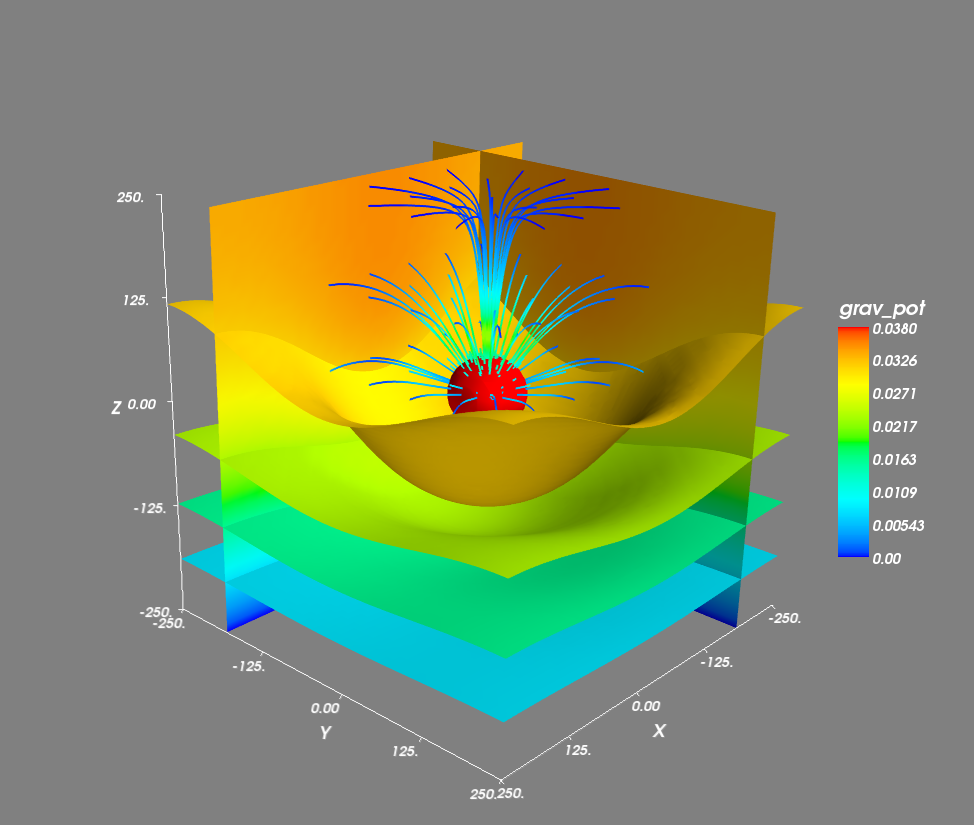
\includegraphics[width=0.75\textwidth]{figures/ex10bpot.png}
\caption{Gravity well with iso surfaces and streamlines of the vector
gravitational potential \textemdash small model.}
\label{fig:ex10bpot}
\end{figure}

\begin{figure}[htp]
\centering
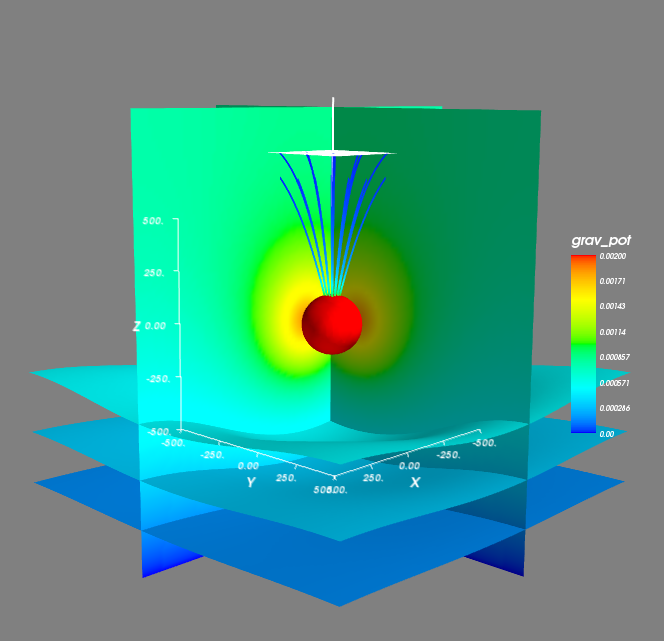
\includegraphics[width=0.75\textwidth]{figures/ex10bpot2.png}
\caption{Gravity well with iso surfaces and streamlines of the vector
gravitational potential \textemdash large model.}
\label{fig:ex10bpot2}
\end{figure}

\begin{figure}[htp]
\centering
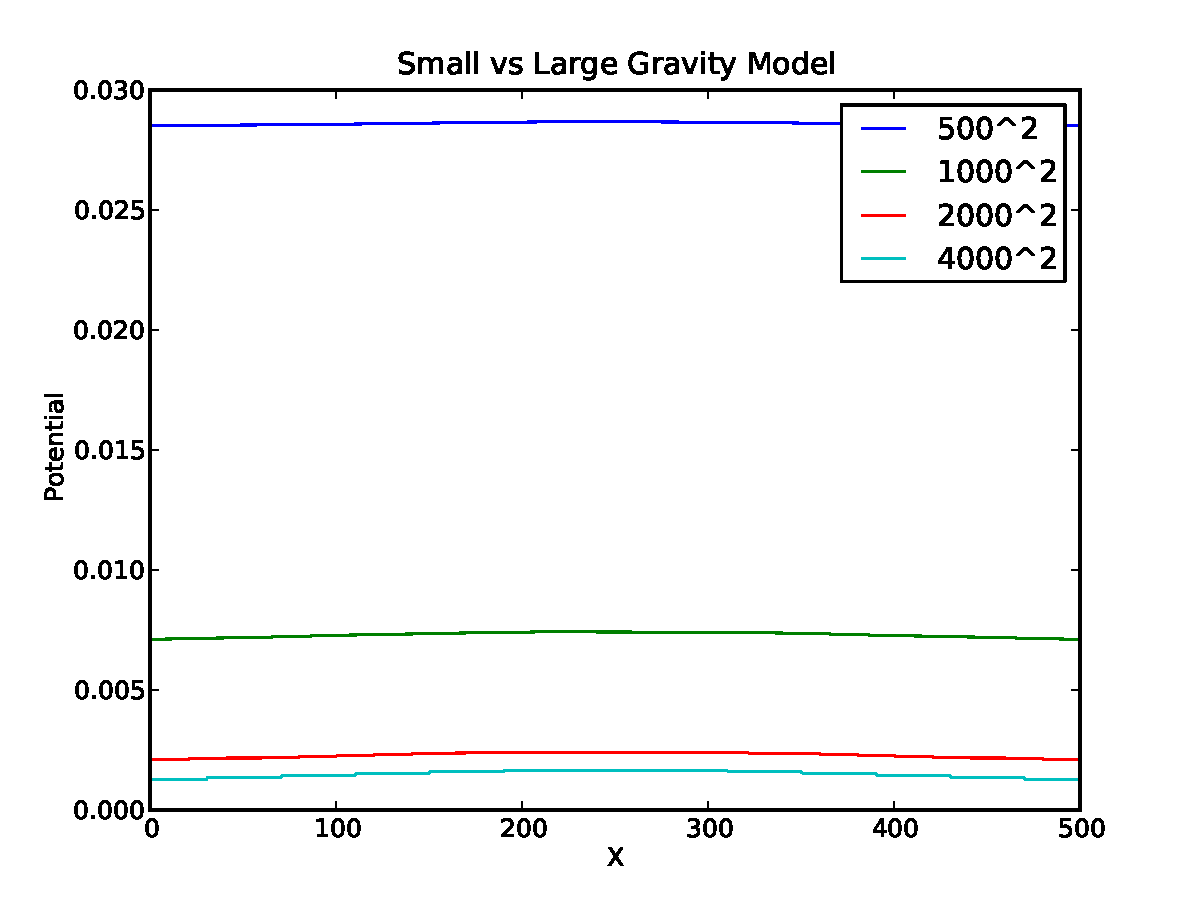
\includegraphics[width=0.85\textwidth]{figures/ex10p_boundeff.pdf}
\caption{Profile of the gravitational profile along x where $y=0,z=250$ for
various sized domains.}
\label{fig:ex10p}
\end{figure}
\clearpage

% \section{Gravity Surface over a fault model.}
% \sslist{example10c.py,example10m.py}
% This model demonstrates the gravity result for a more complicated domain which
% contains a fault. Additional information will be added when geophysical boundary
% conditions for a gravity scenario have been established.
% 
% \begin{figure}[htp]
% \centering
% \subfigure[The geometry of the fault model in example10c.py.]
% 	{\label{fig:ex10cgeo}
% 	 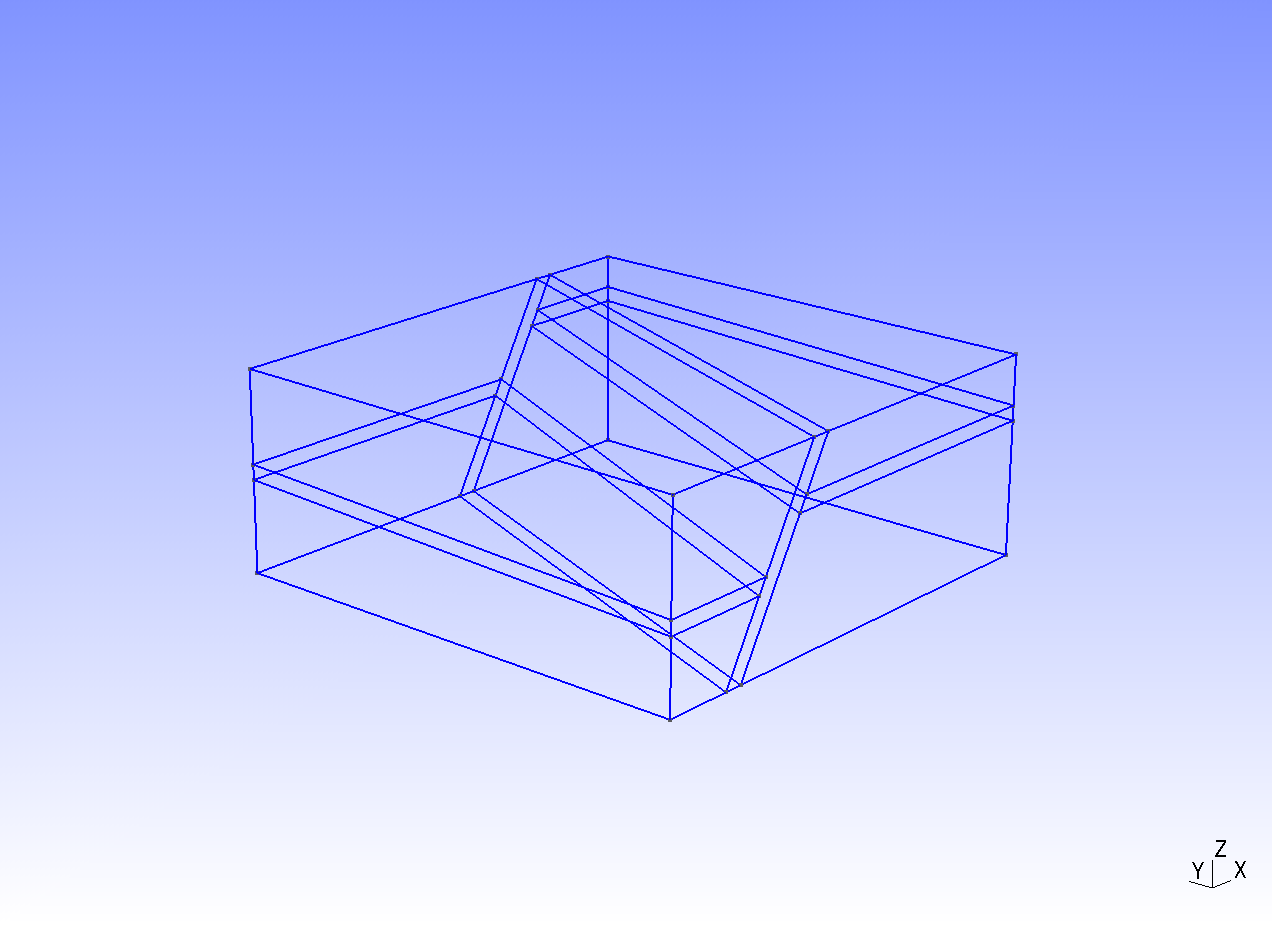
\includegraphics[width=0.8\textwidth]{figures/ex10potfaultgeo.png}} \\
% \subfigure[The fault of interest from the fault model in
% 	example10c.py.] 
% 	{\label{fig:ex10cmsh}
% 	 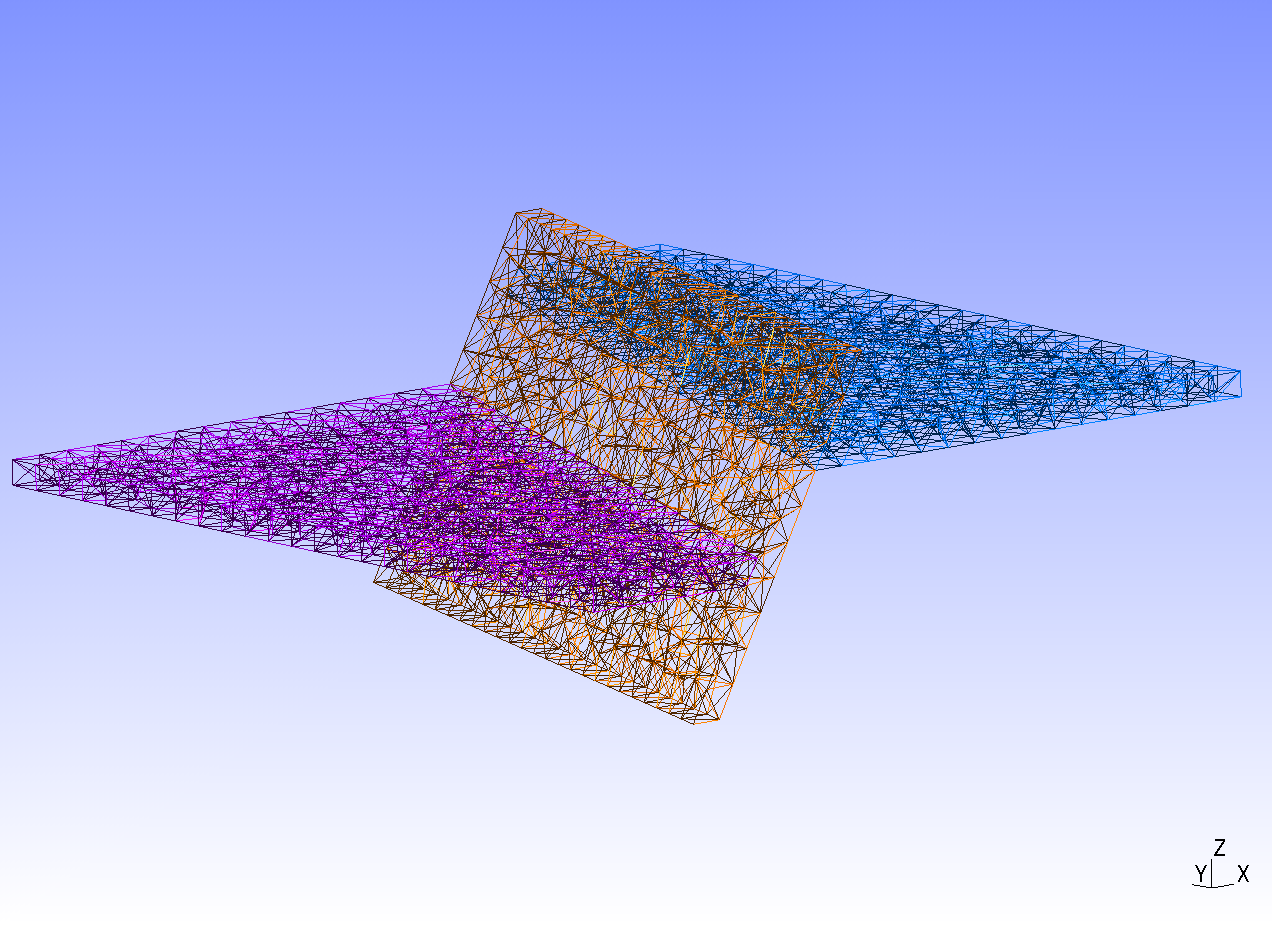
\includegraphics[width=0.8\textwidth]{figures/ex10potfaultmsh.png}}
% \end{figure}
% 
% \begin{figure}[htp]
% \centering
% 	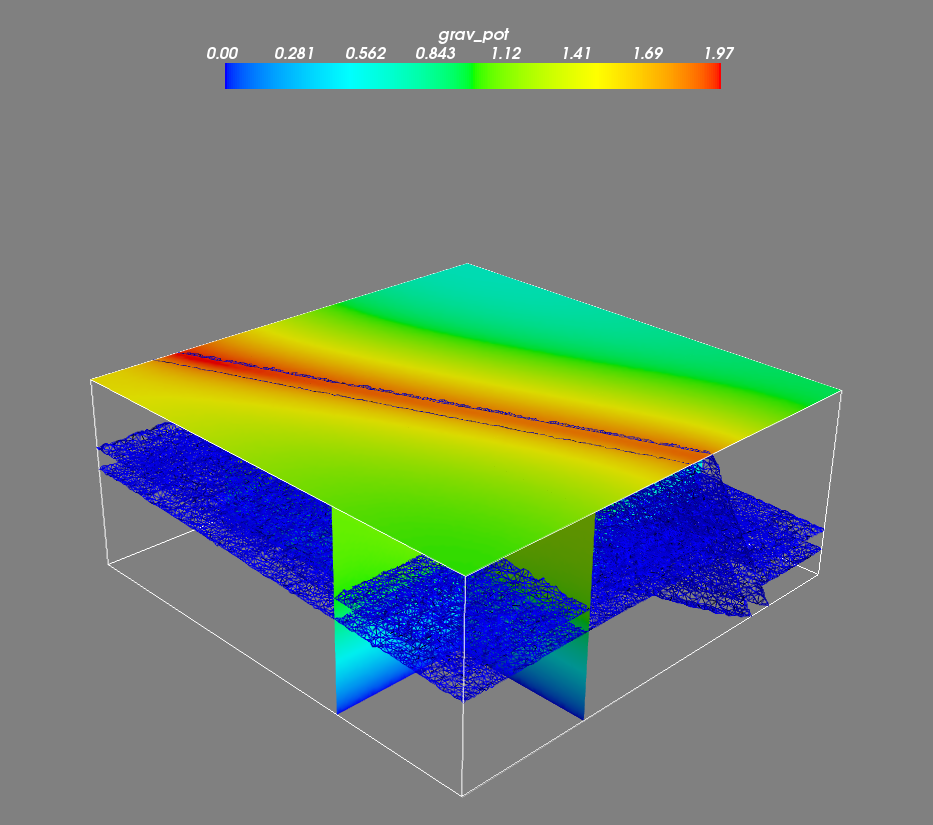
\includegraphics[width=0.8\textwidth]{figures/ex10cpot.png}
% 	\caption{Gravitational potential of the fault model with primary layers and
% 	faults identified as isosurfaces.}
% 	\label{fig:ex10cpot}
% \end{figure}
% \clearpage

\section{Variable mesh-element sizes}
\sslist{example10m.py}
We saw in a previous section that the domain needed to be sufficiently
large for the boundary conditions to be satisfied. This can be troublesome when
trying to solve problems that require a dense mesh, either for solution
resolution of stability reasons. The computational cost of solving a large
number of elements can be prohibitive.S

With the help of Gmsh, it is possible to create a mesh for \esc, which has a
variable element size. Such an approach can significantly reduce the number of
elements that need to be solved, and a large domain can be created that has
sufficient resolution close to the source and extends to distances large enough
that the infinity clause is satisfied.

To create a variable size mesh, multiple meshing domains are required. The
domains must share points, boundaries and surfaces so that they are joined; and
no sub-domains are allowed to overlap. Whilst this initially seems complicated,
it is quite simple to implement. 

This example creates a mesh which contains a high resolution sub-domain at its
center. We begin by defining two curve loops which describe the large or
big sub-domain and the smaller sub-domain which is to contain the high
resolution portion of the mesh. 
\begin{python}
################################################BIG DOMAIN
#ESTABLISHING PARAMETERS
width=10000.    #width of model
depth=10000.    #depth of model
bele_size=500.  #big element size
#DOMAIN CONSTRUCTION
p0=Point(0.0,    0.0)
p1=Point(width, 0.0)
p2=Point(width, depth)
p3=Point(0.0,   depth)
# Join corners in anti-clockwise manner.
l01=Line(p0, p1)
l12=Line(p1, p2)
l23=Line(p2, p3)
l30=Line(p3, p0)

cbig=CurveLoop(l01,l12,l23,l30)

################################################SMALL DOMAIN
#ESTABLISHING PARAMETERS
xwidth=2000.0   #x width of model
zdepth=2000.0   #y width of model
sele_size=10.   #small element size
#TRANSFORM
xshift=width/2-xwidth/2
zshift=depth/2-zdepth/2
#DOMAIN CONSTRUCTION
p4=Point(xshift, zshift)
p5=Point(xwidth+xshift, zshift)
p6=Point(xwidth+xshift, zdepth+zshift)
p7=Point(xshift,    zdepth+zshift)
# Join corners in anti-clockwise manner.
l45=Line(p4, p5)
l56=Line(p5, p6)
l67=Line(p6, p7)
l74=Line(p7, p4)

csmall=CurveLoop(l45,l56,l67,l74)
\end{python}
The small sub-domain curve can then be used to create a surface.
\begin{python}
ssmall=PlaneSurface(csmall)
\end{python}
However, so that the two domains do not overlap, when the big sub-domain
curveloop is used to create a surface it must contain a hole. The hole is
defined by the small sub-domain curveloop.
\begin{python}
sbig=PlaneSurface(cbig,holes=[csmall])
\end{python}
The two sub-domains now have a common geometry and no over-laping features as
per \autoref{fig:ex10mgeo}. Notice, that both domains have a normal in the
same direction.

The next step, is exporting each sub-domain individually, with an appropriate
element size. This is carried out using the \pycad Design command.
\begin{python}
# Design the geometry for the big mesh.
d1=Design(dim=2, element_size=bele_size, order=1)
d1.addItems(sbig)
d1.addItems(PropertySet(l01,l12,l23,l30))
d1.setScriptFileName(os.path.join(save_path,"example10m_big.geo"))
MakeDomain(d1)

# Design the geometry for the small mesh.
d2=Design(dim=2, element_size=sele_size, order=1)
d2.addItems(ssmall)
d2.setScriptFileName(os.path.join(save_path,"example10m_small.geo"))
MakeDomain(d2)
\end{python}
Finally, a system call to Gmsh is required to merge and then appropriately
mesh the two sub-domains together.
\begin{python}
# Join the two meshes using Gmsh and then apply a 2D meshing algorithm.
# The small mesh must come before the big mesh in the merging call!!@!!@!
sp.call("gmsh -2 "+
        os.path.join(save_path,"example10m_small.geo")+" "+
        os.path.join(save_path,"example10m_big.geo")+" -o "+
        os.path.join(save_path,"example10m.msh"),shell=True)
\end{python}
The ``-2'' option is responsible for the 2D meshing, and the ``-o'' option
provides the output path. The resulting mesh is depicted in
\autoref{fig:ex10mmsh}

To use the Gmsh ``*.msh'' file in the solution script, the mesh reading function
``ReadGmsh'' is required. It can be imported via;
\begin{python}
from esys.finley import ReadGmsh
\end{python}
To read in the file the function is called 
\begin{python}
domain=ReadGmsh(os.path.join(mesh_path,'example10m.msh'),2) # create the domain
\end{python}
where the integer argument is the number of domain dimensions.
% 
 \begin{figure}[ht]
\centering
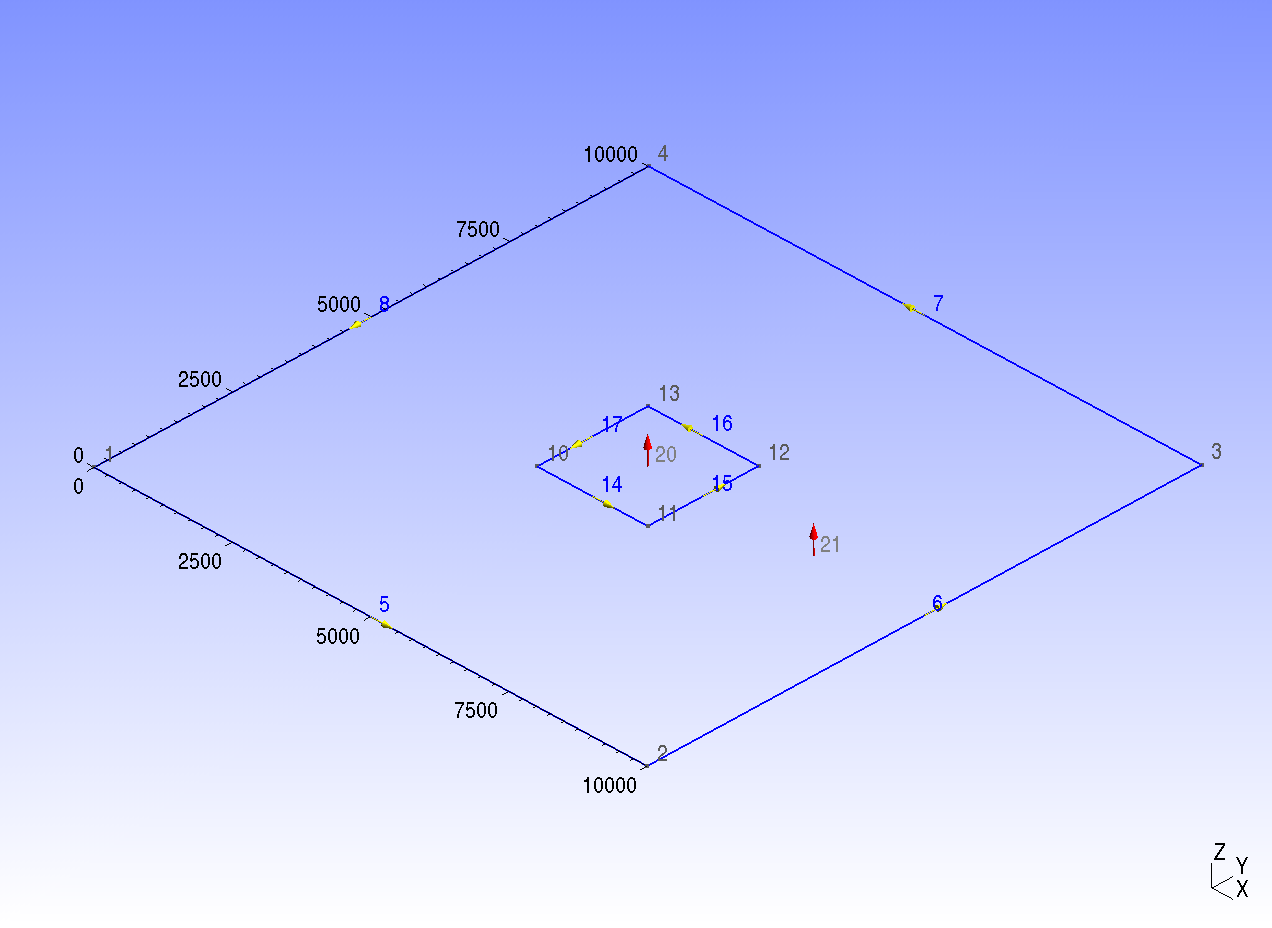
\includegraphics[width=0.8\textwidth]{figures/ex10m_geo.png}
\caption{Geometry of two surfaces for a single domain.}
\label{fig:ex10mgeo}
\end{figure}

\begin{figure}[ht]
\centering
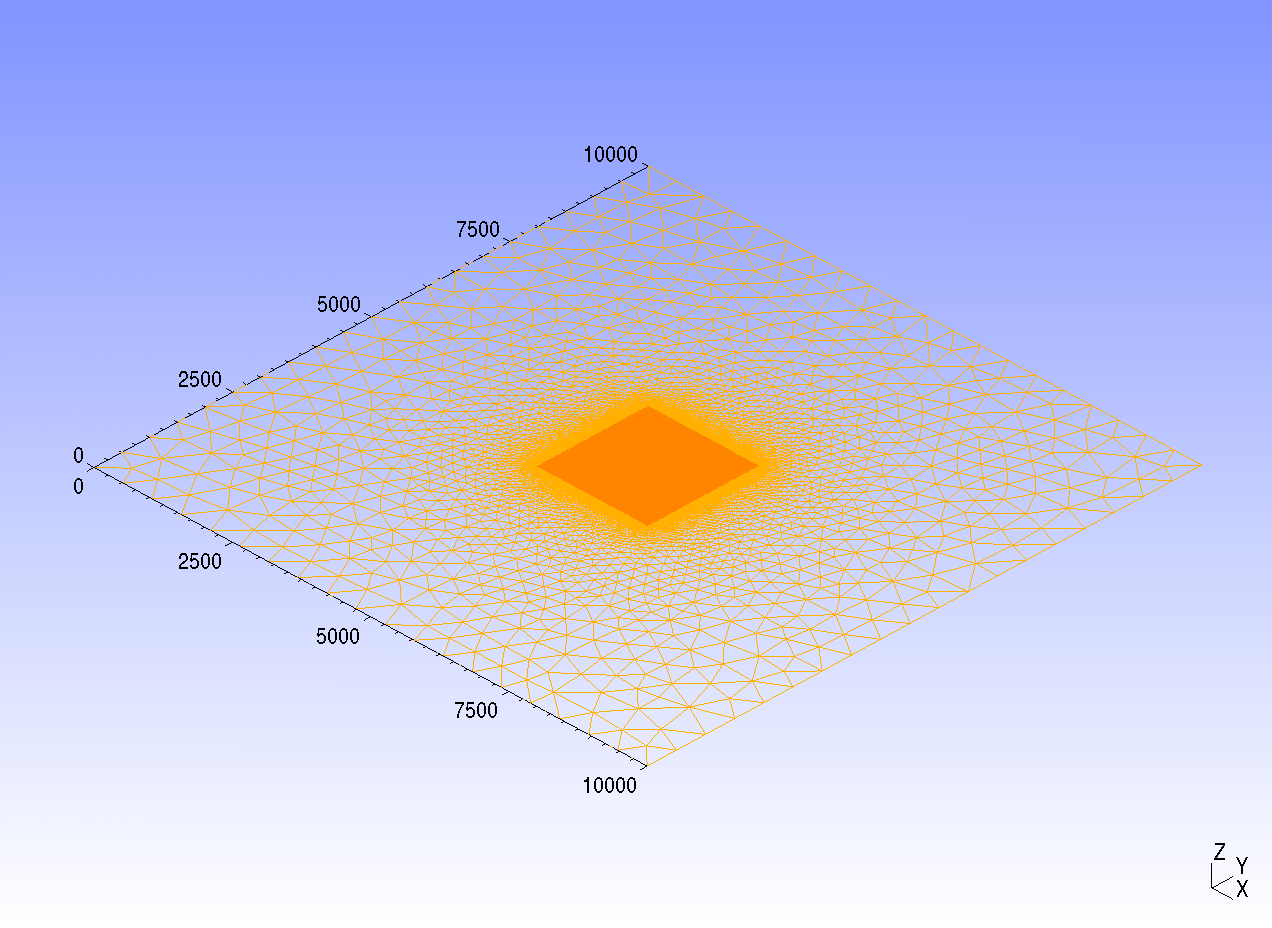
\includegraphics[width=0.8\textwidth]{figures/ex10m_msh.png}
\caption{Mesh of merged surfaces, showing variable element size. Elements
range from 10m in the centroid to 500m at the boundary.}
\label{fig:ex10mmsh}
\end{figure}
\clearpage

\section{Unbounded problems}
With a variable element-size, it is now possible to solve the potential problem
over a very large mesh. To test the accuracy of the solution, we will compare
the \esc result with the analytic solution for the vertical gravitational
acceleration $g_z$ of an infinite horizontal cylinder.

For a horizontal cylinder with a circular cross-section with infinite strike,
the analytic solution is give by
\begin{equation}
g_z = 2\gamma\pi R^2 \Delta\rho \frac{z}{(x^2+z^2)} 
\end{equation}
where $\gamma$ is the gravitational constant (as defined previously), $R$ is the
radius of the cylinder, $\Delta\rho$ is the density contrast and $x$ and $z$ are
geometric factors, relating the observation point to the center of the source
via the horizontal and vertical displacements respectively.

The accuracy of the solution was tested using a square domain. For each test the
dimensions of the domain were modified, being set to 5, 10, 20 and 40 Km. The
results are compared with the analytic solution and are depicted in
\autoref{fig:ex10q boundeff} and \autoref{fig:ex10q boundeff zoom}. Clearly, as
the domain size increases, the \esc approximation becomes more accurate at
greater distances from the source. The same is true at the anomaly peak, where
the variation around the source diminishes with an increasing domain size.

\begin{figure}[ht]
\centering
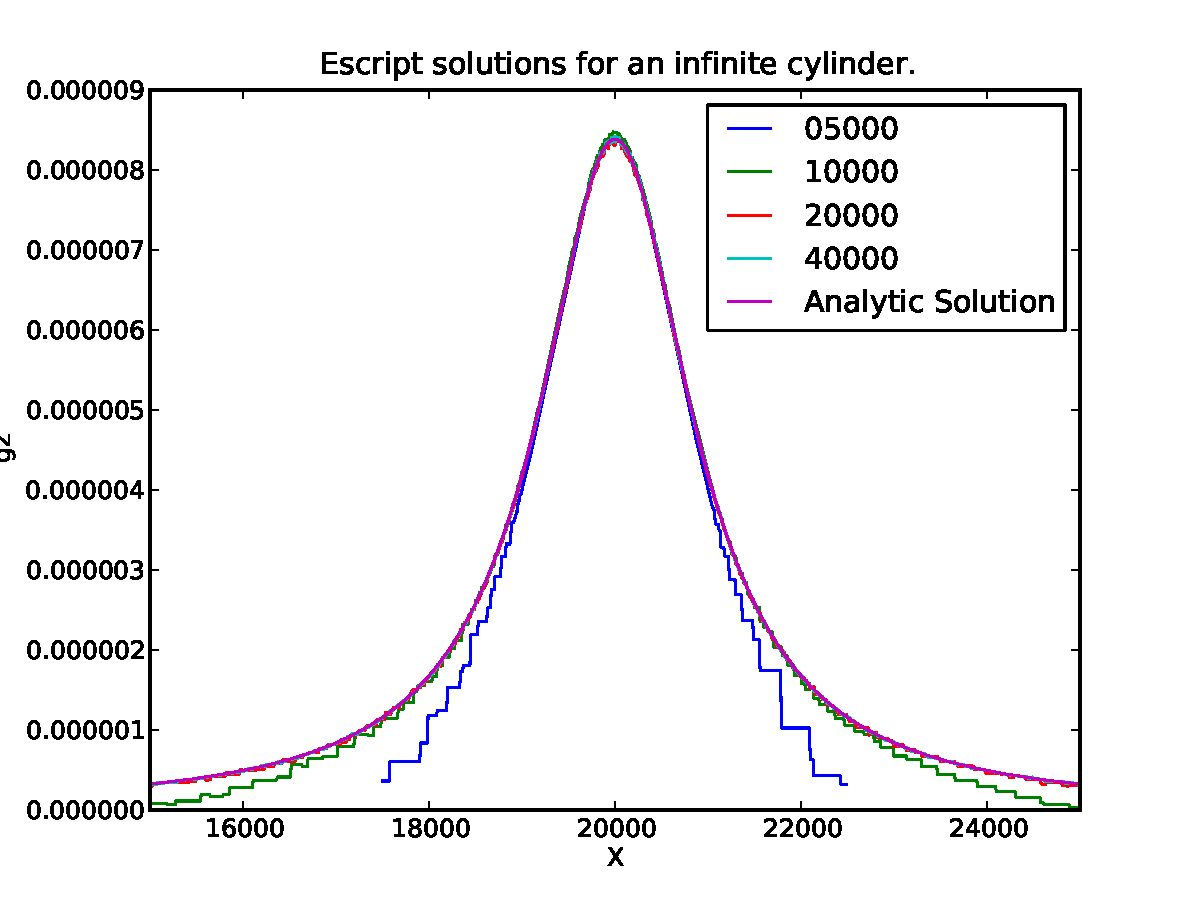
\includegraphics[width=0.8\textwidth]{figures/ex10q_boundeff.pdf}
\caption{Solution profile 1000.0 meters from the source as the domain size
increases.}
\label{fig:ex10q boundeff}
\end{figure}

\begin{figure}[ht]
\centering
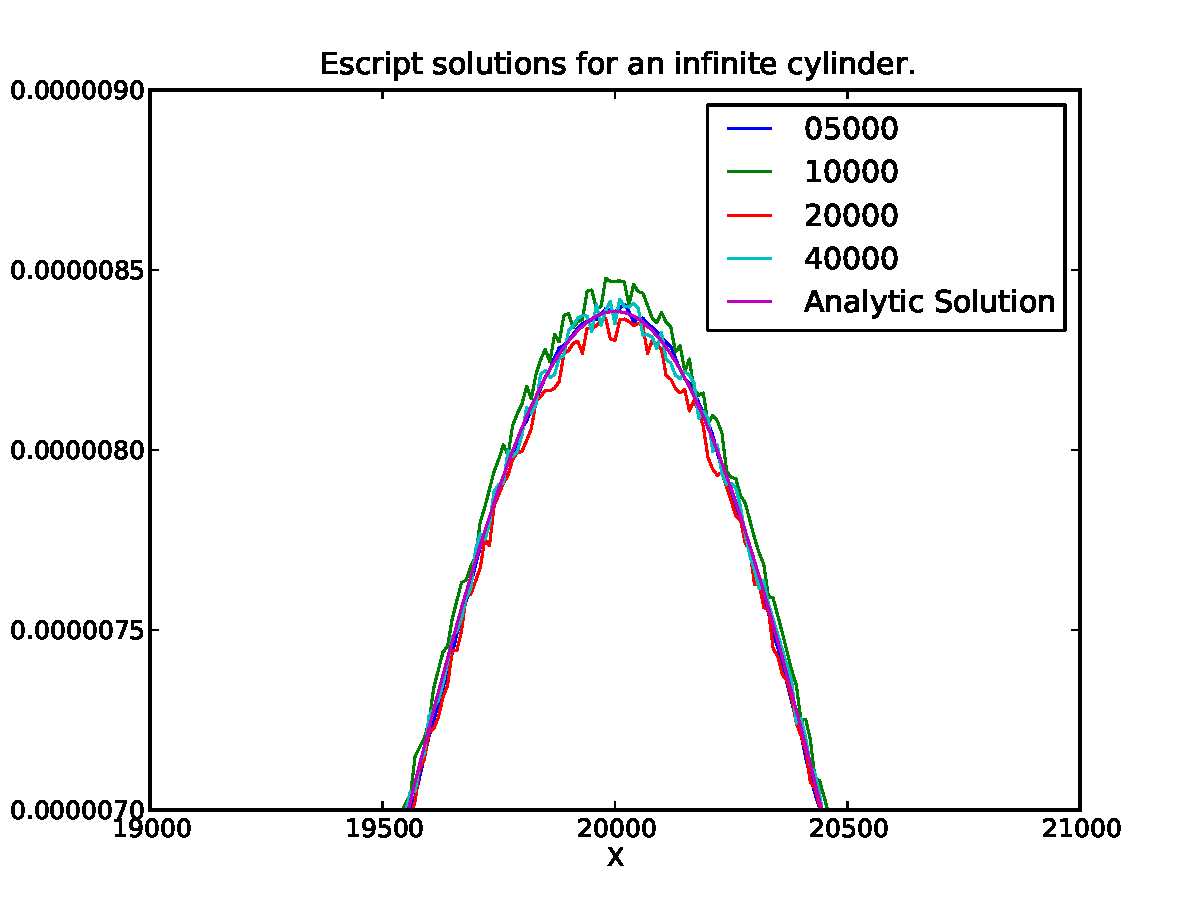
\includegraphics[width=0.8\textwidth]{figures/ex10q_boundeff_zoom.pdf}
\caption{Magnification of \autoref{fig:ex10q boundeff}.}
\label{fig:ex10q boundeff zoom}
\end{figure}

There is a methodology which can help establish an appropriate zero mass region
to a domain. 
\clearpage
